% Manuscript. Target: Journal of Chemical Theory and Computation (achemso class, journal=jctcce).
% Build: latexmk -pdf main.tex (if the bibliography is not found from another directory, set BIBINPUTS=.:). Figures: python paper/make_figures.py, paper/analysis/accuracy_budget.py,
% paper/analysis/tolerance_curve.py, paper/quantum/decision_cost.py, paper/quantum/ae_demo.py (repo root).
% The previous J. Phys. Chem. A draft is kept as main_jpca_draft.tex.
% Items marked \todo{...} need data or a decision before submission.
\documentclass[journal=jctcce,manuscript=article,layout=twocolumn]{achemso}

\usepackage{amssymb}
\usepackage{amsmath}
\usepackage[version=4]{mhchem}
\usepackage{siunitx}
\usepackage{booktabs}
\usepackage{graphicx}
\usepackage{xcolor}
\newcommand{\todo}[1]{\textcolor{red}{[TODO: #1]}}
\newcommand{\kisc}{k_\mathrm{ISC}}
\newcommand{\Hso}{\hat H_\mathrm{SO}}
\newcommand{\aso}{\alpha_\mathrm{SO}}

\author{Parfait Atchade-Adelomou}
\affiliation[MIT Media Lab]{City Science, MIT Media Lab, Massachusetts Institute of Technology,
  75 Amherst St, Cambridge, MA 02139, USA}
\email{parfait@mit.edu}

\title[Accuracy budget and quantum cost of photosensitizer screening]
{How Accurate Must Excited States Be to Screen Triplet Photosensitizers? An Accuracy Budget, a
 Gap-Resolved Intersystem-Crossing Observable, and Decision-Level Quantum Resource Estimates}

\abbreviations{PDT, ISC, SOC, QSVT, QAE, MLAE, CAS, MLJ, THC}
\keywords{photosensitizers, BODIPY, intersystem crossing, accuracy budget, quantum algorithms, QSVT,
amplitude estimation, resource estimation}

\begin{document}

\begin{tocentry}
\todo{TOC graphic: tolerance curve (accuracy budget) next to decision-cost curve.}
\end{tocentry}

% ---------------------------------------------------------------------------------------------
\begin{abstract}
Quantum algorithms have been proposed for screening triplet photosensitizers, but it has not been
asked how accurate the excited-state energies must be for the screening decision to be right, nor what
that decision costs on a fault-tolerant computer. We address both for boron-dipyrromethene (BODIPY)
dyes with measured photophysics. With a Marcus--Levich--Jortner model, a factor-2 intersystem-crossing
(ISC) rate requires singlet--triplet gaps accurate to about 0.08~eV, and to 0.016~eV through a
near-resonant upper triplet, as for the top candidate of a screening round. A B3LYP/$\Delta$SCF pipeline
meets this budget for the iodinated compact dyes but not for the one $\pi$-extended dye with a measured
rate. A (12e,11o) window of canonical orbitals has a summed dipyrrin $\pi$ weight of only 2.5--6.7 out of
11; in an AVAS-selected $\pi$ space, SA-CASSCF/SC-NEVPT2/def2-SVP still overestimates the measured
S$_1$--T$_1$ gaps by about 0.35~eV. We implement the golden-rule rate as a QSVT spectral filter, verify it,
and show that on bare active-space energies it ranks the dyes wrongly. Taking the pipeline rates as
targets, a decision with tensor-hypercontraction qubitization needs $10^{3}$--$10^{6}$ calls of about
$1.5\times10^{8}$ Toffolis, because the rate is a small fraction of the spin--orbit block-encoding norm:
$10^{11}$ Toffolis for light-atom negatives and up to $10^{15}$ near the triplet-yield threshold, with
amplitude estimation cheaper than sampling in every case. When one channel dominates, phase estimation
of its energy with amplitude estimation of its coupling is about ten times cheaper than the filter.
\end{abstract}

% ---------------------------------------------------------------------------------------------
\section{Introduction}

Triplet photosensitizers absorb light and cross efficiently from their singlet to their triplet
manifold. They are the working component of photodynamic therapy (PDT), where the triplet forms
cytotoxic singlet oxygen~\cite{Agostinis2011,Hamblin2004,Wainwright2017,Cieplik2018}, of energy-transfer
photocatalysis~\cite{StriethKalthoff2018,Grosskopf2022}, triplet--triplet annihilation
upconversion~\cite{SinghRachford2010,Bharmoria2020} and theranostics~\cite{Awuah2012,Kowada2015,Wang2024BODIPY};
the inverse process underlies thermally activated delayed fluorescence~\cite{Uoyama2012,Wong2017,Yang2017TADF}.
Design decisions hinge on the energy of the absorbing singlet and on the intersystem-crossing (ISC)
rate, which depends on singlet--triplet gaps and spin--orbit couplings
(SOC)~\cite{Marian2012,Marian2021,Penfold2018,Zhao2013}.
Boron-dipyrromethene (BODIPY) dyes are a common scaffold for these applications, because their
absorption can be shifted to the red by aza substitution or $\pi$-extension and their ISC switched on
by heavy atoms~\cite{Loudet2007,Kamkaew2013,Zhao2015BODIPY}.

Computational screening of such dyes is established, both with high-throughput TDDFT~\cite{GomezBombarelli2016}
and, more recently, with active learning~\cite{Chen2025,Fallani2026}. Quantum computing has been
proposed as the next step. Zhou \emph{et al.}~\cite{Zhou2026PRA} described fault-tolerant algorithms for
PDT photosensitizers in which absorption in a therapeutic window is a QSVT threshold projection of the
dipole-excited state, and ISC is an evolution proxy $\lvert\langle\mathrm{T}_1\rvert
e^{-i\Hso t}\lvert\mathrm{S}_1\rangle\rvert^2$ that contains the SOC but no energy gap; they reported
177--353 logical qubits and $10^{7}$--$10^{9}$ Toffoli gates per shot for active spaces of 11--45
orbitals, and noted that the proxy is a relative quantity to be calibrated. Related proposals outline a golden-rule ISC rate within a relativistic Hamiltonian
workflow~\cite{Zak2026}, and variational calculations have benchmarked BODIPY excitation energies
against experiment~\cite{Nykanen2024}. The underlying primitives are known: smooth functions of the
Hamiltonian estimated through spectral filters and block encodings~\cite{Roggero2019,Roggero2020,Rall2020,Lu2021}
with QSVT~\cite{Gilyen2019,Martyn2021,Low2019}, Hamiltonian factorizations that reduce the cost of
qubitization~\cite{Babbush2018,Berry2019,vonBurg2021,Lee2021,Loaiza2023BLISS,Rocca2024,Caesura2025}, and
amplitude estimation with and without phase
estimation~\cite{Brassard2002,Suzuki2020,Grinko2021,AaronsonRall2020,GiurgicaTiron2022,RallFuller2023,KnillOrtizSomma2007,Montanaro2015}.
End-to-end estimates that include the measurement stage have been made for observables beyond the
energy~\cite{Steudtner2023,Apel2025} and for photochemical yields and rates~\cite{Eklund2026}. On the
classical side, bare active spaces miss the excitation energies of BODIPY and cyanine dyes without
dynamic correlation~\cite{Momeni2015,Chibani2013,BerraudPache2020}, TDDFT overestimates
them~\cite{Jacquemin2012,LeGuennic2015}, and $\Delta$SCF corrects the lowest
states~\cite{Kowalczyk2011,Hait2021}; ISC rates are routinely computed with golden-rule
approaches~\cite{Etinski2011,Baryshnikov2017,deSouza2019,Shi2022}. Perspectives on quantum advantage in
chemistry stress that the target accuracy and the classical baseline must be
stated~\cite{Babbush2021,LeeS2023,Chan2024,Liu2022}.

These proposals leave three questions open, and they are the subject of this work.
\begin{enumerate}
  \item \emph{What accuracy does the screening decision require?} Resource estimates usually target
        chemical accuracy in a fixed active space~\cite{Reiher2017,vonBurg2021,Lee2021,Goings2022,Caesura2025},
        but the accuracy that matters is the one at which the decision (in the window or not; efficient
        ISC or not) stops changing. We derive this accuracy budget from a validated rate model and
        compare it with what classical and active-space methods deliver.
  \item \emph{Does the observable contain the right physics?} ISC rates depend on the gap through the
        Franck--Condon weighted density of states, and in several of our dyes an upper triplet near
        resonance controls the rate. We implement a gap-resolved observable, the golden-rule rate written as a
        spectral filter~\cite{Roggero2020,Rall2020}, verify it in simulation and test what it gives on
        active-space energies.
  \item \emph{What does a decision cost?} Published estimates give costs per shot. A screening
        campaign needs a decision per molecule at a stated confidence. Following end-to-end accountings
        that include the measurement stage~\cite{KnillOrtizSomma2007,Steudtner2023,Eklund2026}, we estimate
        the cost of that decision, including the number of circuit calls.
\end{enumerate}

Our answers rest on a benchmark against measured absorption maxima, singlet--triplet gaps, ISC rates
and triplet yields of BODIPY dyes~\cite{Ly2021}, and on six screening candidates without experimental
data. We do not propose a new quantum algorithm: the spectral-filter primitive and amplitude estimation
are known. Our contributions are (C1) the accuracy budget and the general recipe to derive it, (C2) an
implemented, verified and costed gap-resolved ISC observable, (C3) decision-level resource estimates,
as Eklund \emph{et al.}~\cite{Eklund2026} made for photochemical yields, and (C4) an experimental
benchmark of ISC rates and triplet yields, which previous BODIPY benchmarks of quantum methods did not
include~\cite{Nykanen2024,Genin2025}, with a check of what the (12e,11o) active space of these resource
estimates contains.

% ---------------------------------------------------------------------------------------------
\section{Methods}

\subsection{Classical pipeline}

\paragraph{Geometries and excited states.} Structures are generated from SMILES (with explicit E/Z
labels) with RDKit and MMFF94~\cite{Halgren1996} and optimized with GFN2-xTB~\cite{Bannwarth2019}.
Ground states use B3LYP~\cite{Becke1993,Stephens1994}/def2-SVP~\cite{Weigend2005} in
PySCF~\cite{Sun2020} with density fitting and an effective core potential for iodine. Singlets are
obtained by full TDDFT with an in-house Davidson solver~\cite{Stratmann1998} and triplets by the
Tamm--Dancoff approximation. Because TDDFT overestimates S$_1$ of cyanine-like dyes by several tenths of
an eV~\cite{Momeni2015,LeGuennic2015}, the S$_1$ and T$_1$ energies are replaced with $\Delta$SCF
values: T$_1$ from an unrestricted $M_S=1$ calculation and S$_1$ from the spin-purified sum
rule~\cite{Ziegler1977} with a mixed determinant converged by the maximum-overlap
method~\cite{Gilbert2008}. Higher states keep their TDDFT energies.

\paragraph{Spin--orbit coupling and rates.} SOC is computed with an effective one-electron operator
whose per-element scale factor reproduces the atomic valence spin--orbit constant in the same basis
(e.g.\ \SI{28}{cm^{-1}} for C, \SI{5069}{cm^{-1}} for I), in the spirit of effective nuclear
charges~\cite{Koseki1992}; it reproduces the El-Sayed rules~\cite{ElSayed1963} in formaldehyde. For
iodine the scalar-relativistic effective core potential has no spin--orbit part, and the scaled operator
acts on pseudo-valence orbitals, so the atomic fit corrects their $\langle r^{-3}\rangle$ only on average. This model has
not yet been benchmarked against a standard SOC treatment for these dyes \todo{SOMF or X2C benchmark of
$V_1$ for I2-BDP and $V_2$ for I2-BDP-0}, so the measured rates are its only test. The ISC
rate is the golden rule with a Marcus--Levich--Jortner (MLJ) Franck--Condon weighted density of
states~\cite{Jortner1976}, summed over all triplets:
\begin{equation}
  \kisc = \sum_n \frac{2\pi}{\hbar} V_n^2\,\rho(\Delta E_n),\qquad
  \rho(\Delta E) = \sum_{v=0}^{\infty} \frac{e^{-S}S^v}{v!}
  \frac{1}{\sqrt{4\pi\lambda_s k_BT}}
  \exp\!\left[-\frac{(\Delta E + \lambda_s + v\hbar\omega)^2}{4\lambda_s k_BT}\right],
  \label{eq:mlj}
\end{equation}
with $V_n^2=\sum_M\lvert\langle\mathrm{S}_1\rvert\Hso\lvert\mathrm{T}_n,M\rangle\rvert^2$,
$\Delta E_n=E(\mathrm{T}_n)-E(\mathrm{S}_1)$, $\lambda_s=0.10$~eV, $\hbar\omega=0.17$~eV and $S=0.8$,
set a priori. The gaps are vertical, at the ground-state geometry, whereas the MLJ expression assumes
adiabatic gaps; the difference is of the order of the budget below. The radiative rate follows from the oscillator strength~\cite{Strickler1962}; the
internal-conversion rate is fixed at $k_\mathrm{ic}=1.5\times10^{8}$~s$^{-1}$, the value measured for the
parent BDP~\cite{Ly2021}, for all dyes. This is an approximation: the measured value for I2-BDP is 3.6
times larger, the aza-BODIPYs decay faster, and the computed $k_r$ of BDP and I2-BDP are 1.6--2.4 times the
measured ones. The triplet yield is $\Phi_T=\kisc/(\kisc+k_r+k_\mathrm{ic})$.

\subsection{Accuracy budget}
\label{sec:budget-method}

For every dye we perturb the computed S$_1$--T$_n$ gaps by $\delta$ and recompute $\kisc$ and $\Phi_T$
with eq~\ref{eq:mlj}, keeping SOC, $k_r$ and $k_\mathrm{ic}$ fixed. Two error models are used: all
triplets shifted together relative to S$_1$ (an S--T gap error), and only T$_2$, T$_3$, \dots\ shifted
(an error in the upper triplets). The tolerance for an allowed factor $F$ is the largest $\lvert\delta\rvert$
for which $\kisc$ stays within a factor $F$ of its unperturbed value for every smaller error of either
sign. The class margin is the smallest $\lvert\delta\rvert$ that moves $\Phi_T$ across 0.5. The
absorption margin is the distance of S$_1$ from the nearest edge of the 650--850~nm window.

We use $F=2$ as the reference because the pipeline reproduces the measured $\kisc$ of I2-BDP and
I3-BDP within that factor (Section~\ref{sec:baseline}), and report the tolerance as a function of $F$ and
of $\lambda_s$ (Section~\ref{sec:budget}).

\subsection{Gap-resolved ISC observable}
\label{sec:filter-method}

The golden-rule rate of eq~\ref{eq:mlj}, summed over all triplets and spin components, is an
expectation value of a function of the Hamiltonian,
\begin{equation}
  \kisc = \frac{2\pi}{\hbar}\,\langle\chi\rvert\,\rho(\hat H - E_{\mathrm{S}_1})\,\lvert\chi\rangle,\qquad
  \lvert\chi\rangle = \Hso\lvert\mathrm{S}_1\rangle ,
  \label{eq:filter}
\end{equation}
where $\rho$ acts on the triplet sectors. This is the spectral-filter form of
refs~\citenum{Roggero2020,Rall2020}. We implement it with QSVT: an even Chebyshev polynomial
$P(x)\approx\sqrt{\rho(\alpha\lvert x\rvert + E_c - E_{\mathrm{S}_1})/\rho_\mathrm{max}}$ is applied to the
block-encoded $(\hat H-E_c)/\alpha$, with $E_c$ below the spectrum so that $x\ge0$ and an even polynomial
suffices; the real part is obtained from a linear combination of two QSVT sequences with phases
$\pm\phi$ (\texttt{qml.QSVT} with \texttt{PCPhase} projectors). The success probability of the circuit
is $\langle\chi\rvert P^2\lvert\chi\rangle/\langle\chi\vert\chi\rangle$, which gives $\kisc$ after
multiplication by $(2\pi/\hbar)\langle\chi\vert\chi\rangle\rho_\mathrm{max}$. Each $M_S$ sector of the
active-space Hamiltonian is block-encoded in a randomly rotated basis, and phases are computed by
fixed-point iteration. The code is \texttt{psscreen/isc\_filtered.py}.

\subsection{Decision-level cost model}
\label{sec:decision-method}

On a fault-tolerant machine $\lvert\chi\rangle$ is produced by a block encoding of the one-body
$\Hso$, whose normalization is $\aso=\tfrac12\sum_k\lvert\mu_k\rvert$, with $\mu_k$ the eigenvalues of
the spin-orbital SOC matrix (one basis rotation diagonalizes it). One call of the circuit then succeeds
with probability
\begin{equation}
  p = \kisc/K',\qquad K' = \frac{2\pi}{\hbar}\,\aso^2\,\rho_\mathrm{max},
  \label{eq:p}
\end{equation}
where $\rho_\mathrm{max}$ is the maximum of $\rho$ in eq~\ref{eq:mlj}, the same constant that normalizes
the filter polynomial of eq~\ref{eq:filter}, and $K'$ is known exactly from the Hamiltonian. If $K'$ is below the threshold rate the class is decided
without any call. We consider two decisions per dye, each at confidence 0.95: (D1) $\kisc$ to a relative
statistical error $r=0.2$, which uses about a quarter of the factor-2 budget in $\ln k$ and leaves the
rest to systematic gap errors; and (D2) whether $\Phi_T>0.5$, that is whether $\kisc>k_r+k_\mathrm{ic}$.

The cost of one call for the (12e,11o) active space with tensor-hypercontraction (THC)
qubitization is $C = C_{\mathrm{S}_1} + C_\mathrm{SO} + d\,C_\mathrm{walk}$. $C_\mathrm{walk}=2.97\times10^{3}$
Toffolis per walk step comes from PennyLane's THC estimator (Section~\ref{sec:resources}). The filter
degree $d=(0.55\ln(1/\varepsilon)-0.11)\,\lambda'/\Delta$ is fitted to our own Chebyshev filters, with
$\Delta=\sqrt{2\lambda_sk_BT}$ the MLJ width, polynomial precision $\varepsilon=r\sqrt p/4$, and
$\lambda'=\lambda+\lvert E_0-c_0\rvert=19.4$~Ha the normalization of the shifted operator ($c_0$ is the
identity coefficient); a direct evaluation at the precisions used gives degrees 7--10\% higher than the fit.
S$_1$ is prepared as a spin-adapted sum of $10^{4}$ configuration state functions (an assumption), so that
the triplet components that a spin-free eigenstate filter cannot reject are absent by construction, followed
by an eigenstate filter for a 0.5~eV S$_1$--S$_2$ gap ($C_{\mathrm{S}_1}=2.2\times10^{7}$ Toffolis). The filter
succeeds with probability $\gamma^2$, the overlap of the trial state with S$_1$ (assumed 0.5); its flag is
part of the good state, so the estimators see $\gamma^2p$ and the number of calls scales as $1/\gamma$. One
phase estimation of $E(\mathrm{S}_1)$ to 0.5~mHa ($4\times10^{8}$ Toffolis, a fifth of the factor-2 gap
budget) fixes the filter centre once per dye.

The number of calls is computed for three estimators: direct sampling of the success flag, with the
Dagum--Karp--Luby--Ross stopping rule for D1~\cite{Dagum2000} and Wald's sequential test for
D2~\cite{Wald1945}; maximum-likelihood amplitude estimation (MLAE)~\cite{Suzuki2020}, which needs neither
phase estimation nor a controlled walk, with the empirical constant of a simulation on the filter circuit
(SI Figure~S3); and canonical amplitude estimation~\cite{Brassard2002} with its rigorous bound
(power-of-two grid, median of 16 runs). MLAE is the optimistic estimate and canonical estimation the
rigorous one. The D2 call counts assume that the margin to the threshold is known. As a baseline we also
cost a channel-resolved route: phase estimation of each triplet that carries at least 1\% of $\kisc$, and
amplitude estimation of its coupling $V_n^2$ through a T$_n$ eigenstate filter whose width is the distance to
the nearest other triplet, with the golden rule then evaluated classically. The inputs are the pipeline
values of $\kisc$, $k_r$ and $k_\mathrm{ic}$ and $\aso$ of the canonical window with B3LYP orbitals, so the
costs are those of a machine that would reproduce the pipeline rates; a factor 10 in $\kisc$ changes the D1
cost by a factor of about 3. The cost model is \texttt{paper/quantum/decision\_cost.py}.

\subsection{Active-space references and resources}

To bound what an exact solver of the active-space problem would deliver, we computed CASCI and
strongly contracted NEVPT2~\cite{Angeli2001} singlet and triplet energies (S$_1$, T$_1$, T$_2$) in
(12e,11o) active spaces with PySCF. SA-CASSCF averages the three lowest singlets with equal weights, and
the triplets are CASCI roots on these singlet-optimized orbitals. Two active spaces are compared: the
canonical window of 6 occupied and 5 virtual orbitals around the Fermi level, the usual choice, and a
space selected by a fixed rule (script \texttt{run\_pi\_cas.py}):
the molecule is rotated so that the 11 dipyrrin atoms (two pyrrole rings and the meso atom) lie in the
$xy$ plane, the occupied and virtual RHF orbitals are projected separately on the MINAO 2p$_z$ functions
of these atoms, as in AVAS~\cite{Sayfutyarova2017}, and the 6 occupied and 5 virtual orbitals with the
largest projection are kept. For every active space we report the weight of each orbital on the dipyrrin
$\pi$ space and on iodine. Fault-tolerant resources are estimated with PennyLane's THC qubitization
estimator for the (12e,11o) Hamiltonian of the BODIPY core, with the one-norm taken from double
factorization ($\lambda=15.9$~Ha) and THC rank 22, both assumed rather than computed, with the precision rules
of ref~\citenum{Zhou2026PRA} (20 coefficient bits, 27 rotation bits) and different batchings of the
Givens-rotation angles. All quantum algorithms were run in PennyLane~\cite{Bergholm2018} on a
state-vector simulator.

\subsection{Experimental data}

The benchmark uses the BODIPY core~\cite{Schmitt2009}; 1,3,5,7-tetramethyl-8-phenyl BODIPY (BDP), its
$p$-iodophenyl (I-BDP), 2,6-diiodo (I2-BDP) and triiodo (I3-BDP) derivatives and three 3,5-distyryl
derivatives (BDP-0, I-BDP-0, I2-BDP-0), all measured in toluene by Ly \emph{et al.}~\cite{Ly2021}; and
tetraphenyl aza-BODIPY (aza-BDP-Ph$_4$)~\cite{Killoran2002,Gorman2004,Loudet2008}. \todo{Re-check every
experimental value against Table 2 of ref~\citenum{Ly2021}; aza-BDP-Ph$_4$ values from secondary tables
differ by 5~nm.} Six heavy-atom candidates from a first screening round (Cl2-BDP, Br2-BDP, I1-BDP and
three halogenated aza-BODIPYs) have no experimental data and are used only in the budget and cost analyses.

% ---------------------------------------------------------------------------------------------
\section{Results}

\subsection{Classical baseline}
\label{sec:baseline}

\paragraph{Absorption.} After the $\Delta$SCF correction the six compact dyes lie slightly to the red of
experiment, with a mean error of $-0.055$~eV and a standard deviation of 0.02~eV (Table~\ref{tab:abs},
Figure~S1); uncorrected TDDFT places them 0.35--0.76~eV too high. Vertical energies are
compared with band maxima and solvent is neglected, so we claim that the protocol works for compact
BODIPYs, not that it is general. The same vertical-to-measured comparison is used for every method in this
paper. For BODIPYs the vertical energy and the band maximum, and the vertical and adiabatic gaps, typically
differ by 0.1--0.2~eV~\cite{Momeni2015,Chibani2013}, so part of the pipeline's agreement may come from
error cancellation and part of the larger errors of other methods from the comparison itself.
\todo{Estimate both corrections for BDP and I2-BDP from S$_1$ and T$_1$ optimizations and apply them to all
methods.} It does not transfer to the $\pi$-extended distyryl dyes, whose S$_1$ is
0.21--0.23~eV too low.

\begin{table}
  \caption{Lowest singlet excitation: TDDFT+$\Delta$SCF (B3LYP/def2-SVP, gas phase) versus
  experimental absorption maxima. Distyryl dyes: (E,E) isomers.}
  \label{tab:abs}
  \begin{tabular}{lrrrrr}
    \toprule
    Dye & $\lambda_\mathrm{calc}$ (nm) & $\lambda_\mathrm{exp}$ (nm) & $E_\mathrm{calc}$ (eV) &
    $E_\mathrm{exp}$ (eV) & error (eV) \\
    \midrule
    BODIPY core     & 507 & 503 & 2.45 & 2.46 & $-0.02$ \\
    BDP             & 517 & 503 & 2.40 & 2.46 & $-0.07$ \\
    I-BDP           & 519 & 505 & 2.39 & 2.46 & $-0.06$ \\
    I2-BDP          & 548 & 537 & 2.26 & 2.31 & $-0.05$ \\
    I3-BDP          & 551 & 539 & 2.25 & 2.30 & $-0.05$ \\
    aza-BDP-Ph$_4$  & 678 & 650 & 1.83 & 1.91 & $-0.08$ \\
    \midrule
    BDP-0           & 705 & 628 & 1.76 & 1.97 & $-0.22$ \\
    I-BDP-0         & 708 & 631 & 1.75 & 1.96 & $-0.21$ \\
    I2-BDP-0        & 730 & 644 & 1.70 & 1.93 & $-0.23$ \\
    \bottomrule
  \end{tabular}
\end{table}

\paragraph{ISC.} The computed S$_1$--T$_1$ gaps of BDP (0.72~eV) and I2-BDP (0.61~eV) agree with the
measured 0.77 and 0.59~eV (Table~\ref{tab:isc}). Without heavy atoms $\kisc$ is negligible, as observed.
Iodination at the 2,6 positions gives $\kisc=6.9\times10^{9}$~s$^{-1}$ for I2-BDP ($3.5\times10^{9}$
measured) and $7.1\times10^{9}$~s$^{-1}$ for I3-BDP ($3.9\times10^{9}$ measured), through the
S$_1\to$T$_1$ channel. These two dyes, with nearly identical chemistry, are the only test of the factor-2
agreement, and it depends on the functional: with PBE0 the I2-BDP gap is 0.71~eV and
$\kisc=1.6\times10^{9}$~s$^{-1}$, with BHandHLYP 1.14~eV and $1.8\times10^{6}$~s$^{-1}$ (SI). It also
depends on how the upper triplets are treated. Uncorrected TDDFT gives $\kisc=3\times10^{11}$~s$^{-1}$ for
I2-BDP and $\Phi_T=0.47$ for BDP, where no ISC is observed, and shifting T$_2$ and higher like S$_1$ gives
$\Phi_T=0.56$ for BDP; only the construction used here, with T$_{n\ge2}$ shifted like T$_1$, is consistent
with the compact dyes. Varying $\lambda_s$ between 0.05 and 0.2~eV and $S$ between 0.5 and 1.2 moves
$\kisc$(I2-BDP) between $1.7\times10^{9}$ and $2.5\times10^{10}$~s$^{-1}$, while the ratio to BDP stays
above $10^{11}$.

\begin{table}
  \caption{Triplet photophysics (B3LYP/$\Delta$SCF). $V_1$ is the S$_1$--T$_1$ SOC; rates in s$^{-1}$.
  Experimental values in toluene from ref~\citenum{Ly2021}; ``n.o.'' = not observed. $^a$Secondary sources,
  CHCl$_3$.}
  \label{tab:isc}
  \begin{tabular}{lcccccc}
    \toprule
    Dye & $\Delta E_\mathrm{ST}$ calc/exp (eV) & $V_1$ (cm$^{-1}$) & $\kisc$ calc & $\kisc$ exp &
    $\Phi_T$ calc & $\Phi_T$ exp \\
    \midrule
    BODIPY core    & 0.71 / --    & 0.00 & $2\times10^{-2}$ & --  & 0.00 & $\approx0$ \\
    BDP            & 0.72 / 0.77  & 0.00 & $1\times10^{-2}$ & n.o. & 0.00 & n.o. \\
    I-BDP          & 0.72 / 0.76  & 0.00 & 2.9 & -- & 0.00 & -- \\
    I2-BDP         & 0.61 / 0.59  & 13.2 & $6.9\times10^{9}$ & $3.5\times10^{9}$ & 0.95 & 0.84 \\
    I3-BDP         & 0.61 / 0.58  & 13.5 & $7.1\times10^{9}$ & $3.9\times10^{9}$ & 0.95 & 0.81 \\
    aza-BDP-Ph$_4$ & 0.73 / --    & 0.10 & $1.4\times10^{5}$ & -- & 0.00 & low$^a$ \\
    \midrule
    I2-BDP-0       & 0.50 / --    & 0.43 & $1.7\times10^{7}$ & $4.5\times10^{8}$ & 0.04 & 0.76 \\
    \bottomrule
  \end{tabular}
\end{table}

\paragraph{The distyryl failure.} For I2-BDP-0 the pipeline gives
$\kisc=1.7\times10^{7}$~s$^{-1}$, 26 times below experiment, and $\Phi_T=0.04$ instead of 0.76. In the
uncorrected TDDFT spectrum T$_2$ lies 0.08~eV above S$_1$ with 8~cm$^{-1}$ of SOC, which gives
$\kisc=1.1\times10^{9}$~s$^{-1}$ and $\Phi_T=0.67$, close to experiment. The $\Delta$SCF step lowers
S$_1$ and T$_1$ but not T$_2$, moves T$_2$ 0.51~eV above S$_1$ and closes that channel. Conformers do not
explain the discrepancy ($\kisc$ varies by less than a factor of 1.5), and a different hybrid
functional does not fix it: with PBE0 the compact dyes are within 0.00 to $+0.05$~eV and $\kisc$ of
I2-BDP and I3-BDP is $1.6\times10^{9}$~s$^{-1}$, but I2-BDP-0 stays at $7.6\times10^{6}$~s$^{-1}$
because T$_2$ remains 0.44~eV above S$_1$. Across the treatments we have, T$_2$ lies 0.08~eV (uncorrected B3LYP), 0.12~eV
(BHandHLYP/$\Delta$SCF), 0.44~eV (PBE0/$\Delta$SCF), 0.51~eV (B3LYP/$\Delta$SCF) and 0.54~eV
(canonical-window SA-CASSCF/SC-NEVPT2) above S$_1$. The $\Delta$SCF entries share one construction, and the
canonical window of this dye holds little of its $\pi$ system (Table~\ref{tab:window}). If S$_1$ is instead
anchored to experiment, T$_2$ comes within 0.1--0.2~eV of it. The position of T$_2$ is therefore uncertain by
about 0.4~eV, 25 times the near-resonance tolerance of Section~\ref{sec:budget}, and our calculations do not
explain why ISC is fast in this dye. Besides a near-resonant T$_2$, candidate explanations, none tested here, are relaxation of S$_1$ along the distyryl
torsions, which can change the adiabatic ordering; spin--vibronic coupling to T$_2$; a T$_1$ channel
with a larger SOC at the S$_1$ geometry; and solvent effects. The pipeline's S$_1$ is also least reliable
for this dye ($-0.23$~eV, Table~\ref{tab:abs}). What the case does show is that $\Phi_T$ moves between
0.04 and 0.67 depending on where T$_2$ lies within half an eV of S$_1$, so a screening method must place
the upper triplets of $\pi$-extended dyes within the budget of Section~\ref{sec:budget}, and that none of
the methods we used reproduces the measured rate. We also note that unlabeled
styryl double bonds were embedded as cis isomers in a first calculation and gave spuriously good
absorption; automated screening of $\pi$-extended dyes must fix and verify the stereochemistry.

\subsection{Accuracy budget}
\label{sec:budget}

\paragraph{ISC rates need gaps to about 0.08~eV.} A 0.1~eV error in the S$_1$--T gaps changes $\kisc$ by
up to a factor of 2.7, because the dominant channel lies in the inverted region of the MLJ curve, where the
rate grows as the gap closes (Figure~\ref{fig:mlj}). Keeping $\kisc$ within a factor of 2 for every error
of either sign requires gap errors below 0.079--0.083~eV for the ISC-active validation dyes and
0.062--0.083~eV over all dyes except azaBDP\_Br2; within a factor of 1.5, below 0.035--0.056~eV; within a factor of 3,
0.12--0.14~eV; within a factor of 10, 0.18--0.38~eV (Figure~\ref{fig:tolcurve}a). The factor-2 tolerance
depends on the assumed reorganization energy, from 0.03--0.07~eV at $\lambda_s=0.05$~eV to
0.09--0.13~eV at $\lambda_s=0.25$~eV (Figure~\ref{fig:tolcurve}b). The tolerance at small $\lambda_s$ partly reflects the resolved
progression of the single-mode model. With independent errors on the two states, 0.08~eV corresponds to
about 2~mHa per state. The gap is not the only input: a factor 2 in $\kisc$ is also $\pm41$\% in $V$, so the
SOC model and the gaps share the same factor of 2.

\paragraph{The triplet-yield class is more forgiving, except near $\Phi_T=0.5$.} The
class ($\Phi_T$ above or below 0.5) does not flip for any gap error up to 0.5~eV in seven of the nine
dyes and needs about 0.4~eV in the other two. It is tight only for dyes near $\Phi_T=0.5$, as for two
screening candidates below, and there it is also set by $k_r+k_\mathrm{ic}$, which the pipeline knows only
to a factor of 2--4.

\paragraph{Window membership is the tightest requirement for red-absorbing dyes.} The dyes that absorb
near the therapeutic window lie 0.00--0.07~eV from its 650~nm edge in experiment; aza-BDP-Ph$_4$ sits on
it and the three distyryl dyes just outside. Their computed S$_1$ lies 0.15--0.21~eV inside, so a sharp
window classifies all three wrongly. A threshold observable inherits this edge sensitivity, and a
smooth, error-aware window score is better suited to screening.

\paragraph{The top screening candidate is the most fragile prediction.} The 2,6-dibromo aza-BODIPY
(azaBDP\_Br2, $\Phi_T=0.97$) owes its rate to an uphill S$_1\to$T$_2$ channel: T$_2$ lies 0.11~eV above
S$_1$ with 47~cm$^{-1}$ of SOC. A 0.1~eV error in that gap changes $\kisc$ by a factor of about 20, the
factor-2 tolerance is 0.016~eV (Figure~\ref{fig:tolcurve}), and $\Phi_T$ drops below 0.5 if T$_2$ is
0.08~eV higher. Moreover T$_2$ keeps its TDDFT energy while S$_1$ is $\Delta$SCF-corrected, the same
inconsistency as in the distyryl dye. Two other candidates (Br2-BDP, azaBDP\_IPh2) sit at
$\Phi_T\approx0.5$, where the class flips for gap errors of 0.01--0.02~eV. A gap-free S$_1$--T$_1$ proxy
would rank azaBDP\_Br2 ($V_1^2=1.8$~cm$^{-2}$) below azaBDP\_IPh2 (26~cm$^{-2}$) and Br2-BDP
(8.6~cm$^{-2}$), the opposite of the golden-rule order.

\begin{figure}
  \centering
  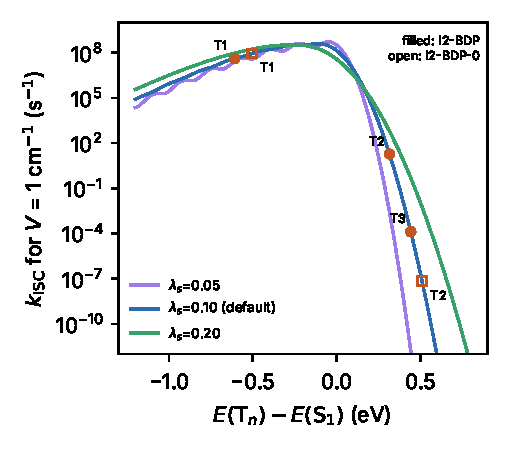
\includegraphics[width=0.48\textwidth]{figures/mlj_gap_sensitivity.pdf}
  \caption{ISC rate of eq~\ref{eq:mlj} for a coupling of 1~cm$^{-1}$ as a function of the
  S$_1$--T$_n$ gap, for three values of $\lambda_s$. Points: the computed T$_1$--T$_3$ channels of I2-BDP
  (filled) and I2-BDP-0 (open), from the TDDFT/$\Delta$SCF pipeline.}
  \label{fig:mlj}
\end{figure}

\begin{figure}
  \centering
  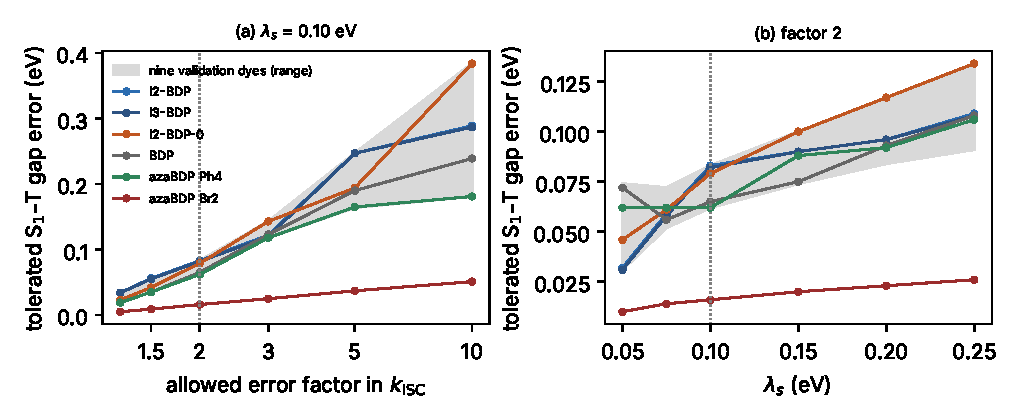
\includegraphics[width=0.95\textwidth]{figures/tolerance_curve.pdf}
  \caption{Accuracy budget. Largest S$_1$--T gap error (all triplets shifted together) that keeps
  $\kisc$ within the allowed factor, (a) as a function of that factor at $\lambda_s=0.10$~eV and (b) for
  a factor of 2 as a function of $\lambda_s$. Grey band: range over the nine validation dyes.}
  \label{fig:tolcurve}
\end{figure}

\subsection{Active-space Hamiltonians against the budget}
\label{sec:cas}

\paragraph{What the (12e,11o) window contains.} The dipyrrin $\pi$ system has 11 atoms and 12
$\pi$ electrons, so a (12e,11o) space can be the $\pi$ space of the chromophore. The canonical window of 6
occupied and 5 virtual orbitals, the simplest way to build an active space of this size, is not
(Table~\ref{tab:window}). Summed over its 11 orbitals, the weight on the dipyrrin 2p$_z$ space is 6.7 for the BODIPY core, 5.2 for BDP, 3.6 for I-BDP, 2.5 for I2-BDP and I3-BDP
and 3.0 for BDP-0. In I2-BDP only HOMO and LUMO are $\pi$ orbitals of the chromophore; four of the eleven
orbitals sit mainly on iodine (lone pairs and C--I $\sigma^*$), and the rest are $\sigma$ orbitals or $\pi$
orbitals of the substituents. For the compact dyes the AVAS selection gives 11 orbitals with dipyrrin $\pi$
weights of at least 0.90 and a clear gap in the projection eigenvalues (at least 0.90 for the orbitals kept,
below 0.1 for the first one rejected), and SA-CASSCF keeps them $\pi$ orbitals (minimum weight 0.89). For
the distyryl dye BDP-0 the gap is less clear (0.85 kept, 0.15 rejected), because its $\pi$ system extends over
27 centres and the dipyrrin space truncates it. The same label
``(12e,11o)'' therefore describes different model chemistries across dyes in the canonical window, but
one model chemistry in the AVAS space.

\begin{table}
  \caption{Character of the (12e,11o) active orbitals: canonical RHF window (HOMO$-5$ to LUMO$+4$) versus
  the AVAS $\pi$ selection. $\sum w_\pi$: weight on the 2p$_z$ space of the 11 dipyrrin atoms, summed over
  the 11 orbitals (11 for a pure $\pi$ space); $n_\mathrm{I}$: orbitals with more than half their weight on
  iodine; $\aso$ in cm$^{-1}$ with Hartree--Fock orbitals.}
  \label{tab:window}
  \footnotesize\setlength{\tabcolsep}{4pt}
  \begin{tabular}{lcccccc}
    \toprule
    & \multicolumn{3}{c}{canonical window} & \multicolumn{3}{c}{AVAS $\pi$ space} \\
    Dye & $\sum w_\pi$ & $n_\mathrm{I}$ & $\aso$ & $\sum w_\pi$ & min $w_\pi$ (SA-CASSCF) & $\aso$ \\
    \midrule
    BODIPY core & 6.7 & 0 & 133   & 10.9 & 0.98 & 8 \\
    BDP         & 5.2 & 0 & 27    & 10.7 & 0.90 & 7 \\
    I-BDP       & 3.6 & 2 & 5579  & 10.7 & 0.90 & 80 \\
    I2-BDP      & 2.5 & 4 & 8315  & 10.6 & 0.89 & 299 \\
    I3-BDP      & 2.5 & 5 & 11421 & 10.6 & 0.89 & 304 \\
    BDP-0       & 3.0 & 0 & 11    & 10.6 & --   & 7 \\
    \bottomrule
  \end{tabular}
\end{table}

\paragraph{A controlled $\pi$ space does not reach the budget either.} In the AVAS $\pi$ space with
SA-CASSCF orbitals and def2-SVP, SC-NEVPT2 places S$_1$ 0.54--0.59~eV above experiment and overestimates the
measured S$_1$--T$_1$ gaps by 0.33--0.37~eV for BDP, I-BDP and I2-BDP (Table~\ref{tab:pi}). BDP and I-BDP share
the same $\pi$ space and agree to 0.02~eV, so these are effectively two independent results. The lowest upper
triplet lies 0.36--0.44~eV above S$_1$, as in the pipeline, so the S$_1\to$T$_2$ channel stays closed. No
orbital is inert: every root has occupations that deviate from 0 or 2 by at least 0.02. Without orbital
optimization, CASCI on the AVAS orbitals misses S$_1$ by 1.2--2.3~eV and NEVPT2 by 0.5--0.9~eV.

These errors are larger than those reported for CASPT2 in a (12e,11o) $\pi$ space with larger basis
sets~\cite{Momeni2015}, which ref~\citenum{Zhou2026PRA} quotes as close to experiment. Three differences can
account for this, and we cannot yet separate them. The def2-SVP basis overestimates excitation energies; a
$\pi$-only reference misses the $\sigma$--$\pi$ polarization that ionic, cyanine-like $\pi\pi^*$ states such as
the BODIPY S$_1$ need, which second-order perturbation theory recovers only in part; and the state averaging
over three singlets, with triplets as CASCI roots on singlet orbitals, is untested. Because T$_1$ relaxes more
than S$_1$, a vertical-to-adiabatic correction would probably increase, not decrease, the gap error.
\todo{def2-TZVP and SA(3S+2T) runs for BDP and I2-BDP on tars; I3-BDP NEVPT2, aza-BDP-Ph$_4$ and the distyryl
dyes still running.} What the data do establish is that a controlled (12e,11o) $\pi$ space with
second-order dynamic correlation in a double-$\zeta$ basis misses the gaps by several times the budget, with a
nearly uniform error.

\begin{table}
  \caption{AVAS $\pi$-space (12e,11o) vertical energies (eV), SA-CASSCF orbitals over three singlets,
  def2-SVP, with experiment. T$_2-$S$_1$: lowest triplet above T$_1$ (SC-NEVPT2 interchanges T$_2$ and T$_3$
  for the first three dyes).}
  \label{tab:pi}
  \begin{tabular}{lccccccc}
    \toprule
    & \multicolumn{3}{c}{CASCI} & \multicolumn{3}{c}{SC-NEVPT2} & exp \\
    Dye & S$_1$ & S$_1-$T$_1$ & T$_2-$S$_1$ & S$_1$ & S$_1-$T$_1$ & T$_2-$S$_1$ & S$_1$ / S$_1-$T$_1$ \\
    \midrule
    BODIPY core & 2.88 & 1.02 & $+0.23$ & 3.00 & 1.05 & $+0.38$ & 2.46 / -- \\
    BDP         & 2.91 & 1.09 & $+0.24$ & 3.01 & 1.10 & $+0.36$ & 2.46 / 0.77 \\
    I-BDP       & 2.90 & 1.10 & $+0.23$ & 3.00 & 1.11 & $+0.36$ & 2.46 / 0.76 \\
    I2-BDP      & 2.87 & 1.00 & $+0.24$ & 2.90 & 0.96 & $+0.44$ & 2.31 / 0.59 \\
    I3-BDP      & 2.86 & 1.01 & $+0.23$ & --   & --   & --      & 2.30 / 0.58 \\
    \bottomrule
  \end{tabular}
\end{table}

\paragraph{Results on the canonical window.} The canonical window gives the same conclusion with
smaller, less systematic errors (Tables~S1--S3, Figure~S2). On RHF orbitals CASCI overestimates S$_1$ by
1.4--2.0~eV, 20--30 times the budget, and NEVPT2 reduces the error to 0.06--0.27~eV. On SA-CASSCF
orbitals NEVPT2 places S$_1$ 0.51--0.79~eV above experiment for the compact dyes, and the S$_1$--T$_1$
gaps of BDP, I-BDP, I2-BDP and I3-BDP are 0.22--0.27~eV too large. A shift of half an eV on an orbital
change is a sign that the character of the window changes; the AVAS results show that the close
agreement on RHF orbitals comes from that mixed character, not from a better reference. For
aza-BDP-Ph$_4$, NEVPT2 places T$_2$ only 0.17~eV above S$_1$ (0.29~eV in the pipeline), a difference larger
than the budget in the quantity that decides whether an upper channel opens. Growing the window from
(8,8) to (14,14) for BDP and I2-BDP lowers the CASSCF S$_1$ by 0.2--0.7~eV; from (8,8) to (12,12) it leaves
the NEVPT2 S$_1$--T$_1$ gap flat (0.96--1.00 and 0.82--0.88~eV against 0.77 and 0.59~eV measured), while T$_2$--S$_1$
moves by 0.24~eV for I2-BDP; the (14,14) step changes nothing, the signature of two inert orbitals
(Table~S3). \todo{(16,16) when it finishes.} Quantum phase estimation on any of these bare Hamiltonians
would reproduce the CASCI energies, so a dynamic-correlation step on top of the quantum calculation is
required.

\subsection{Gap-resolved ISC observable in simulation}
\label{sec:filter}

In CAS(4,4) and CAS(6,6) (6--11 wires per $M_S$ sector, polynomial degrees
3324--8000), the QSVT circuit reproduces the polynomial evaluated on the exact spectrum to all printed
digits and the exact golden-rule rate to within 0.03\% (2\% for the smallest rate, $10^{-10}$ of the
filter maximum, near the dynamic-range floor set by the polynomial error) (Table~\ref{tab:filter}). The
circuit computes the observable it is designed for.

On active-space energies, however, S$_1$ lies
2.3--2.8~eV above T$_1$ instead of about 0.6~eV, so the S$_1\to$T$_1$ channel is closed by the
Franck--Condon factor, and the rate comes from upper triplets that happen to lie within 0.06--0.25~eV
of the misplaced S$_1$. At CAS(6,6) this puts the iodine-free BODIPY core ($2.5\times10^{8}$~s$^{-1}$)
above I2-BDP ($4.2\times10^{6}$~s$^{-1}$), the opposite of experiment. The gap-free proxy ranks the same
dyes correctly, because iodine increases the coupling (11--25 against $\le0.001$~cm$^{-1}$), but for the
wrong reason: it does not see the mechanism, and it fails when an upper triplet controls ISC, as for
azaBDP\_Br2. The filter is the right observable once the Hamiltonian is good enough, which is the
budget of Section~\ref{sec:budget}.

\begin{table}
  \caption{Gap-resolved ISC rate (s$^{-1}$) from the QSVT filter circuit and from the exact golden rule,
  with CASCI energies (the circuit agrees with the same polynomial evaluated on the exact spectrum to all
  printed digits); and the gap-free S$_1$--T$_1$ coupling. $\Delta E$ is the CASCI S$_1$--T$_1$ gap.}
  \label{tab:filter}
  \begin{tabular}{llrrrrr}
    \toprule
    Dye & CAS & degree & $\kisc$ QSVT & $\kisc$ exact & $V_1$ (cm$^{-1}$) & $\Delta E$ (eV) \\
    \midrule
    BODIPY core & (4,4) & 3324 & $1.972\times10^{4}$ & $1.972\times10^{4}$ & $<10^{-3}$ & 2.70 \\
    BODIPY core & (6,6) & 5720 & $2.479\times10^{8}$ & $2.479\times10^{8}$ & $1\times10^{-3}$ & 2.34 \\
    BDP         & (4,4) & 4106 & $3.519\times10^{2}$ & $3.519\times10^{2}$ & $<10^{-3}$ & 2.79 \\
    I2-BDP      & (4,4) & 4492 & $4.568\times10^{-1}$ & $4.680\times10^{-1}$ & 11.49 & 2.36 \\
    I2-BDP      & (6,6) & 8000 & $4.229\times10^{6}$ & $4.230\times10^{6}$ & 24.84 & 2.49 \\
    \bottomrule
  \end{tabular}
\end{table}

\subsection{Fault-tolerant resources, like for like}
\label{sec:resources}

With PennyLane's THC qubitization estimator and the precision rules of ref~\citenum{Zhou2026PRA}, one
walk step for the (12e,11o) BODIPY-core Hamiltonian costs $2.8$--$3.5\times10^{3}$ Toffolis. The qubit
count is set by how the Givens-rotation angles are loaded: 374 wires when all angles are loaded at once,
239 with two batches, 158 with five and 131 with ten, for 10--30\% more Toffolis (THC rank 22; rank 44
gives 136--379). The 177 qubits of ref~\citenum{Zhou2026PRA} for this active space lie in this range, so
qubit counts should be quoted together with the angle-loading choice and compared on Toffolis. The
gap-resolved filter needs about $3\times10^{4}$ walk steps at the MLJ width
($\Delta\approx0.07$~eV), that is about $10^{8}$ Toffolis for the filter itself, the same order as the
$8\times10^{7}$ per shot of the gap-free proxy~\cite{Zhou2026PRA}. With the coherent S$_1$ preparation
included, one call costs $1.4$--$2.1\times10^{8}$ Toffolis on 158 logical qubits. The error of the THC
factorization at rank 22 and of the finite coefficient and rotation precision on the S$_1$--T$_n$ gaps
is not yet included in the budget. \todo{THC rank 22 and 44 S$_1$--T$_1$, S$_1$--T$_2$ gaps of the
BODIPY core against exact CASCI.}

\subsection{Cost of a screening decision}
\label{sec:decision}

\paragraph{The rate is a small fraction of the spin--orbit norm.} For the heavy-atom dyes $\aso$ is
850--12\,400~cm$^{-1}$ in the canonical (12e,11o) window with B3LYP orbitals (Table~\ref{tab:decision}). The
success probability $p=\gamma^2\kisc/K'=\gamma^2(V_\mathrm{eff}/\aso)^2$, with
$V_\mathrm{eff}^2=\sum_nV_n^2\rho(\Delta E_n)/\rho_\mathrm{max}$ the Franck--Condon-weighted coupling, is
$3\times10^{-9}$ to $2\times10^{-5}$ for the ISC-active dyes, and the number of calls, not the cost per call,
dominates. Two factors make $p$ small. For I2-BDP, $\aso/\lVert\chi\rVert=11$ and $\lVert\chi\rVert/V_\mathrm{eff}=270$:
most of the norm of $\Hso\lvert\mathrm{S}_1\rangle$ goes to triplets far from resonance, which the filter
rejects. $\aso$ also depends on the active space: with Hartree--Fock orbitals it is 8300~cm$^{-1}$ in the
canonical window of I2-BDP and 300~cm$^{-1}$ in the AVAS $\pi$ space (Table~\ref{tab:window}). In a planar
$\pi$ space the one-centre SOC between $\pi$ orbitals vanishes; the 300~cm$^{-1}$ come from non-planarity,
polarization functions and multicentre terms, and such a space cannot carry the rate. An active space for the
ISC observable has to include the orbitals that carry the SOC, and the costs below, for a window that holds
iodine orbitals by accident, should be read with that in mind.

\paragraph{Amplitude estimation.} On the actual filter circuit for the BODIPY core (CAS(4,4), $M_S=1$ sector,
$p=5.6\times10^{-6}$), the good-state probability after $m$ Grover iterations follows
$\sin^2((2m+1)\theta)$ to $5\times10^{-10}$ (SI Figure~S3). At the 95th percentile, MLAE reaches 18\% relative
error with $1.0\times10^{5}$ calls; canonical estimation needs $2.6\times10^{5}$, and direct sampling is still at
250\%. These statistics come from the $\sin^2$ law with an ensemble over nearby amplitudes. The MLAE constant
($\varepsilon_\mathrm{rel}\sqrt p\,N_\mathrm{calls}=45$) holds only above about 5\% error, and at the true
amplitude the error stalls at 6--9\%, which we attribute to the grid search of our implementation; we therefore
give the rigorous canonical totals next to the MLAE ones.

\paragraph{Decision costs.} Estimating $\kisc$ to 20\% (D1) costs $6\times10^{12}$--$7\times10^{14}$ Toffolis
with MLAE and $3\times10^{13}$--$6\times10^{15}$ with canonical estimation, $5\times10^{4}$--$4\times10^{6}$ calls
of $1.2$--$1.7\times10^{8}$ Toffolis; direct sampling costs $3\times10^{2}$--$3\times10^{4}$ times more
(Table~\ref{tab:decision}, Figure~\ref{fig:decision}). For the class decision (D2), amplitude estimation is
cheaper than sequential sampling for every dye, by 3--7 times for light-atom negatives and by $10^{2}$--$10^{4}$
for heavy-atom dyes: certifying $p<p_\mathrm{th}$ takes about $1/p_\mathrm{th}$ samples but only about
$1/\sqrt{p_\mathrm{th}}$ amplitude-estimation calls. The cost is set by the distance to the threshold:
$5\times10^{10}$--$5\times10^{11}$ Toffolis for light-atom negatives, $4\times10^{11}$--$2\times10^{13}$ for
heavy-atom dyes far from $\Phi_T=0.5$, and $3$--$4\times10^{14}$ (MLAE) or $1$--$3\times10^{15}$ (canonical)
for Br2-BDP and azaBDP\_IPh2, at 0.94 and 1.2 times the threshold rate. At $10^{6}$ Toffolis per second a D1
estimate for I2-BDP takes about 4.5 years with MLAE, and the deepest single circuit of canonical estimation
has $8\times10^{13}$ Toffolis, which requires logical error rates below about $10^{-14}$ per Toffoli. For a
campaign of $N$ dyes with a family-wise error of 0.05, canonical estimation needs 2.5 times more runs for
$N=100$; for MLAE the tail of the error distribution has not been characterized.

\paragraph{A channel-resolved route is cheaper here.} In every ISC-active dye one channel carries more than
99\% of the rate. Phase estimation of that triplet and amplitude estimation of its coupling through a T$_n$
eigenstate filter, with the golden rule evaluated classically, costs 9--21 times less than the filter for
D1 ($5\times10^{11}$--$8\times10^{13}$ Toffolis), because the success probability is $\gamma^2V_n^2/\aso^2$
rather than $\gamma^2V_\mathrm{eff}^2/\aso^2$ and the eigenstate filter is wider than the MLJ width. It also
keeps the line-shape parameters outside the circuit. The filter is preferable when many triplets contribute
comparably or the channels are not known in advance.

The D1 costs of the filter are $10^{2}$--$10^{5}$ times the $3.8\times10^{10}$ Toffolis of the 483-shot ISC
estimate reported in ref~\citenum{Zhou2026PRA}, for a different dye and Hamiltonian; D2 for light-atom
negatives is comparable to it. The proxy targets a fixed additive precision of a relative, gap-free quantity
and, as its authors note, has to be calibrated before it can take decision D2. Our totals
($5\times10^{10}$--$6\times10^{15}$) overlap the lower end of the range reported for photochemical yields by
Eklund \emph{et al.}~\cite{Eklund2026}, who simulate the dynamics, whereas our line shape is a classical model.

\begin{table}
  \caption{Decision-level cost (Toffolis), (12e,11o) canonical window with B3LYP orbitals, THC
  qubitization (158 logical qubits for the walk), confidence 0.95, pipeline rates as targets, $\gamma^2=0.5$.
  $V_\mathrm{eff}$: Franck--Condon-weighted coupling; $p=\gamma^2\kisc/K'$. D1: $\kisc$ to 20\% with MLAE and
  canonical estimation, and with the channel-resolved route (MLAE), listed for $\kisc\ge10^{6}$~s$^{-1}$; D2:
  is $\Phi_T>0.5$, best estimator. One call costs $1.2$--$1.7\times10^{8}$ Toffolis.}
  \label{tab:decision}
  \scriptsize\setlength{\tabcolsep}{2pt}
  \begin{tabular}{lrrrrrrrr}
    \toprule
    Dye & $\aso$ (cm$^{-1}$) & $V_\mathrm{eff}$ (cm$^{-1}$) & $\kisc/k_\mathrm{th}$ & $p$ &
    D1, MLAE & D1, canonical & D1, channel & D2 \\
    \midrule
    BDP          &    39 & $5\times10^{-6}$ & $3\times10^{-11}$ & $1\times10^{-14}$ & -- & -- & -- & $8.8\times10^{10}$ \\
    I-BDP        &  6553 & $9\times10^{-5}$ & $7\times10^{-9}$  & $9\times10^{-17}$ & -- & -- & -- & $1.5\times10^{13}$ \\
    I2-BDP       & 12006 & 4.2  & 20   & $6.1\times10^{-8}$ & $1.4\times10^{14}$ & $1.3\times10^{15}$ & $1.1\times10^{13}$ & $1.6\times10^{13}$ \\
    I3-BDP       & 12372 & 4.3  & 20   & $6.0\times10^{-8}$ & $1.4\times10^{14}$ & $1.3\times10^{15}$ & $1.1\times10^{13}$ & $1.6\times10^{13}$ \\
    I2-BDP-0     &  2656 & 0.21 & 0.04 & $3.1\times10^{-9}$ & $7.0\times10^{14}$ & $5.8\times10^{15}$ & $7.9\times10^{13}$ & $1.3\times10^{13}$ \\
    Br2-BDP      &  1474 & 0.92 & 0.94 & $1.9\times10^{-7}$ & $7.6\times10^{13}$ & $6.3\times10^{14}$ & $6.0\times10^{12}$ & $2.6\times10^{14}$ \\
    azaBDP\_Br2  &   855 & 5.7  & 35   & $2.2\times10^{-5}$ & $5.8\times10^{12}$ & $3.2\times10^{13}$ & $5.4\times10^{11}$ & $5.9\times10^{11}$ \\
    azaBDP\_IPh2 &  7173 & 1.0  & 1.2  & $1.1\times10^{-8}$ & $3.6\times10^{14}$ & $2.8\times10^{15}$ & $1.7\times10^{13}$ & $4.3\times10^{14}$ \\
    \bottomrule
  \end{tabular}
\end{table}

\begin{figure}
  \centering
  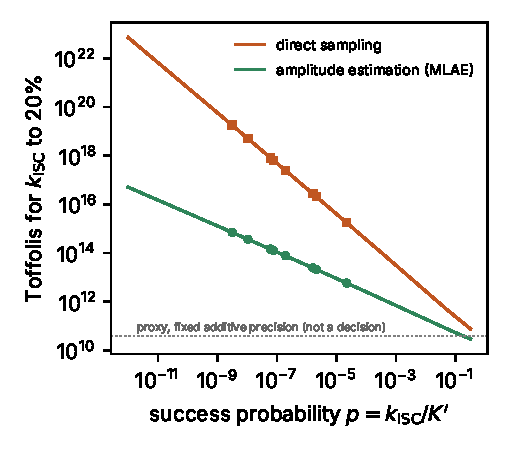
\includegraphics[width=0.48\textwidth]{figures/decision_cost.pdf}
  \caption{Toffolis to estimate $\kisc$ to 20\% at confidence 0.95 as a function of the success
  probability $p=\gamma^2\kisc/K'$, with direct sampling and with MLAE; points are the ISC-active dyes. The dotted
  line is the total of the gap-free proxy of ref~\citenum{Zhou2026PRA} at fixed additive precision, which
  does not correspond to a decision.}
  \label{fig:decision}
\end{figure}

% ---------------------------------------------------------------------------------------------
\section{Discussion}

\paragraph{What the useful quantum target is.} A rate estimate needs singlet--triplet gaps to about
0.08~eV, and to 0.016~eV near resonance, while the triplet-yield class tolerates far more except near its
threshold. A B3LYP/$\Delta$SCF pipeline meets the rate budget for the compact iodinated dyes but not for the
$\pi$-extended dye tested; bare active-space Hamiltonians misplace S$_1$ and the gaps so badly that a
mechanism-correct observable evaluated on them ranks dyes wrongly; and NEVPT2 in a controlled $\pi$ space and
a double-$\zeta$ basis still misses the gaps by several times the budget. We argue that the useful quantum
target is therefore excited-state energies with dynamic correlation at the budget accuracy, evaluated with a
gap-resolved observable, not a larger bare active space or a better gap-free proxy. For the dyes studied here,
where one channel dominates, the cheapest gap-resolved observable is channel-resolved: phase estimation of
the channel energies and amplitude estimation of the couplings. Two qualifications apply. The
active space must be chosen by a controlled rule, since the canonical window mixes $\pi$, $\sigma$ and
iodine orbitals; and an active space for the ISC observable needs orbitals that carry the SOC, which a pure
$\pi$ space does not have in a planar dye (El-Sayed's rule), so the heavy-atom orbitals have to be
included deliberately rather than by accident. Perturbation theory on quantum-computed reduced density
matrices~\cite{Krompiec2022,Takeshita2020}, downfolding~\cite{Huang2023DSRG} and transcorrelated
Hamiltonians~\cite{Motta2020TC,Kumar2022TC} are candidate routes; the measurement cost they add has to fit
the same budget. 

\paragraph{The cost lever is the spin--orbit encoding.} Because amplitude estimation scales as
$1/\sqrt p$ and $p=\gamma^2(V_\mathrm{eff}/\aso)^2$, the decision cost scales as $\aso/V_\mathrm{eff}$, which is
150--$1.3\times10^{4}$ for the ISC-active dyes. Of this, the part $\aso/\lVert\chi\rVert$ (11 for I2-BDP) is
the price of the block encoding and can be reduced by an encoding of $\Hso$ restricted to the couplings that
matter, for example the heavy-atom one-centre terms; the part $\lVert\chi\rVert/V_\mathrm{eff}$ (270 for
I2-BDP) is the off-resonant weight that the filter removes, and only a channel-resolved route avoids it.

\paragraph{A general recipe.} Any screening decision based on a rate model can be treated the same
way: perturb the inputs, find the largest error that leaves the decision unchanged, and compare it with
what the candidate methods deliver, for example the S$_1$--T$_1$ gap of TADF
emitters~\cite{Uoyama2012,Wong2017} or the triplet energy of photocatalysts relative to a
substrate~\cite{StriethKalthoff2018}. The budget sets the target accuracy, and the margin to the decision
boundary sets the measurement cost on a quantum computer.

\paragraph{Limitations.} The benchmark is small: nine dyes from essentially one family and three
measured ISC rates, two of them for nearly identical dyes. The factor-2 agreement holds for B3LYP and not
for PBE0 or BHandHLYP. One basis set (def2-SVP, also for NEVPT2), GFN2-xTB geometries and the gas phase were
used, with one conformer, and all energies are vertical, also as inputs to the MLJ rate. The SOC operator is
an effective one-electron model not yet benchmarked against a standard SOC treatment, and $k_r$ and
$k_\mathrm{ic}$ are uncertain by a factor of 2--4. The controlled $\pi$-space results cover five dyes at
CASSCF, four at NEVPT2 and three with a measured gap. The cost model takes its rates from the pipeline and
$\aso$ from a canonical window, assumes a spin-adapted S$_1$ trial state with overlap 0.5, an assumed THC rank
and one-norm, and an oracle margin for D2, and omits the THC factorization error. The quantum algorithms were
simulated in small active spaces.

% ---------------------------------------------------------------------------------------------
\section{Conclusions}

For BODIPY photosensitizers, a factor-2 ISC rate needs singlet--triplet gaps to about 0.08~eV, and a
near-resonant upper triplet tightens this to 0.016~eV, which makes the top screening candidate the most
fragile prediction. A B3LYP/$\Delta$SCF pipeline meets this budget for compact iodinated dyes; neither it nor
our multireference references explain the one $\pi$-extended dye with a measured rate. Active spaces for
these dyes must be selected by a controlled rule, and a controlled (12e,11o) $\pi$ space with SC-NEVPT2 in
def2-SVP still misses the gaps by several times the budget. A gap-resolved ISC observable is implemented and
verified, and on a fault-tolerant computer a screening decision costs $10^{11}$--$10^{15}$ Toffolis, set by the
spin--orbit normalization and the distance to the threshold, with amplitude estimation cheaper in every case
and a channel-resolved route cheaper still when one channel dominates. The accuracy budget is a general
recipe for setting the target of classical and quantum methods in rate-based screening.

% ---------------------------------------------------------------------------------------------
\begin{acknowledgement}
We thank the Xanadu team, authors of ref~\citenum{Zhou2026PRA}, for their work on fault-tolerant
quantum algorithms for photosensitizer design, which motivated this study.
\end{acknowledgement}

\begin{suppinfo}
Absorption parity plot (Figure~S1); canonical-window CASCI, SA-CASSCF/SC-NEVPT2 and active-space sweep
(Tables~S1--S3, Figure~S2); amplitude-estimation simulation (Figure~S3). \todo{Geometries, per-dye
outputs, accuracy-budget tables for all dyes, decision-cost tables for all dyes.}
\end{suppinfo}

\section*{Data Availability}
\sloppy
Code, geometries and all results: \url{https://github.com/pifparfait/psscreen}. Tables~\ref{tab:abs}
and~\ref{tab:isc} come from the validation runs of \texttt{psscreen}; the budget and
Figure~\ref{fig:tolcurve} from \texttt{paper/analysis/accuracy\_budget.py} and \texttt{tolerance\_curve.py};
Tables~\ref{tab:window}, \ref{tab:pi} and S1--S3 from
\texttt{paper/references/run\_sa\_nevpt2.py NAME}, \texttt{run\_cas\_sweep.py NAME} and
\texttt{run\_pi\_cas.py NAME}; Table~\ref{tab:filter} from \texttt{psscreen/isc\_filtered.py};
Table~\ref{tab:decision} and Figures~\ref{fig:decision} and S3 from
\texttt{paper/quantum/decision\_cost.py}, \texttt{alpha\_so.py} and \texttt{ae\_demo.py}. \todo{Archive a tagged
release on Zenodo and cite the DOI.}

\bibliography{refs,related_work}

\end{document}
